\chapter{الجينوميات والتسلسل}\label{ch:b3:genomics}

نُشر أول جينوم كامل لكائن حر المعيشة، وهو \qty{1.8}{Mb} من بكتيريا،
عام 1995 بعد سنة من عمل فريق من أربعين باحثًا. أما الجينوم البشري،
وقدره \num{3.2} مليار زوج قواعد، فاستغرق اتحادًا دوليًا ثلاث عشرة سنة
ونحو ثلاثة مليارات دولار وأُعلن إنجازه عام 2003. واليوم يقرأ جهاز
على طاولة جينومًا بشريًا في ليلة بمئات قليلة من الدولارات، ويسلسل
مستشفًى ورم مريض ليختار له دواءً، ويستخلص متحف جينوم عظم عمره أربعون
ألف سنة ويقرؤه. وموضوع هذا الفصل التقنية التي أتاحت ذلك،
والرياضيات التي تحوّل ملايين القراءات القصيرة إلى جينوم، وما علّمته
الجينومات المنجزة عن حجم DNA عندنا ومحتواه وتاريخه. أما الفصل الذي
يليه فيتناول الخوارزميات التي تقارن المتتاليات بعد الحصول عليها.

\section{قراءة DNA}

\begin{definition}[التسلسل بإنهاء السلسلة]\label{def:b3:genomics:sanger}
\index{تسلسل سانغر}\index{ثنائي منزوع الأكسجين}\index{إنهاء السلسلة}
\emph{تسلسل سانغر} ينسخ قالبًا مفرد الطاق انطلاقًا من بادئة
ببوليميراز DNA بحضور النوكليوتيدات الأربعة السوية ونسبة صغيرة من
\emph{النوكليوتيدات ثنائية منزوعة الأكسجين}، التي تنقصها الهيدروكسيل
3$'$ فتنهي السلسلة حيثما أُدخلت. ويحمل كل نوكليوتيد ثنائي منزوع
الأكسجين صبغًا متألقًا مختلفًا. والناتج مزيج من القطع، قطعة لكل موضع
من القالب، تنتهي كل منها بقاعدة معلومة الهوية؛ فإذا فُصلت بالحجم
في شعيرة من هلام، مرّت بكاشف مرتبةً بالطول، وكان تسلسل الألوان هو
تسلسل القالب. ويقرأ الشوط الواحد \qtyrange{700}{900}{bp} بمعدل خطأ
دون $10^{-3}$؛ وهو ما يزال الطريقة المعتمدة للتحقق من بنية مركّبة أو
من مورّثة واحدة.
\end{definition}

\begin{proof}[شواهد]
نشر سانغر ونيكلن وكولسون الطريقة عام 1977 واستعملوها في تلك السنة
\omterm{def:b3:genomics:ngs}{لقراءة} \qty{5386}{bp} من العاثية $\phi$X174 --- وهو أول
جينوم DNA كامل --- وعام 1981 \omterm{def:b3:genomics:ngs}{لقراءة} \qty{16569}{bp} من
المتقدرة البشرية. وقرأ فلايشمان وزملاؤه (1995)
\qty{1.83}{Mb} من \emph{Haemophilus influenzae} بتكسير الجينوم
كله إلى قطع عشوائية، وتسلسل \num{24000} منها،
\omterm{def:b3:genomics:assembly}{وتجميع} القراءات بالحاسوب --- وهي استراتيجية \emph{الخردقة الجينومية
الشاملة} التي وسّعها كل مشروع لاحق.
\end{proof}

\begin{omfigure}
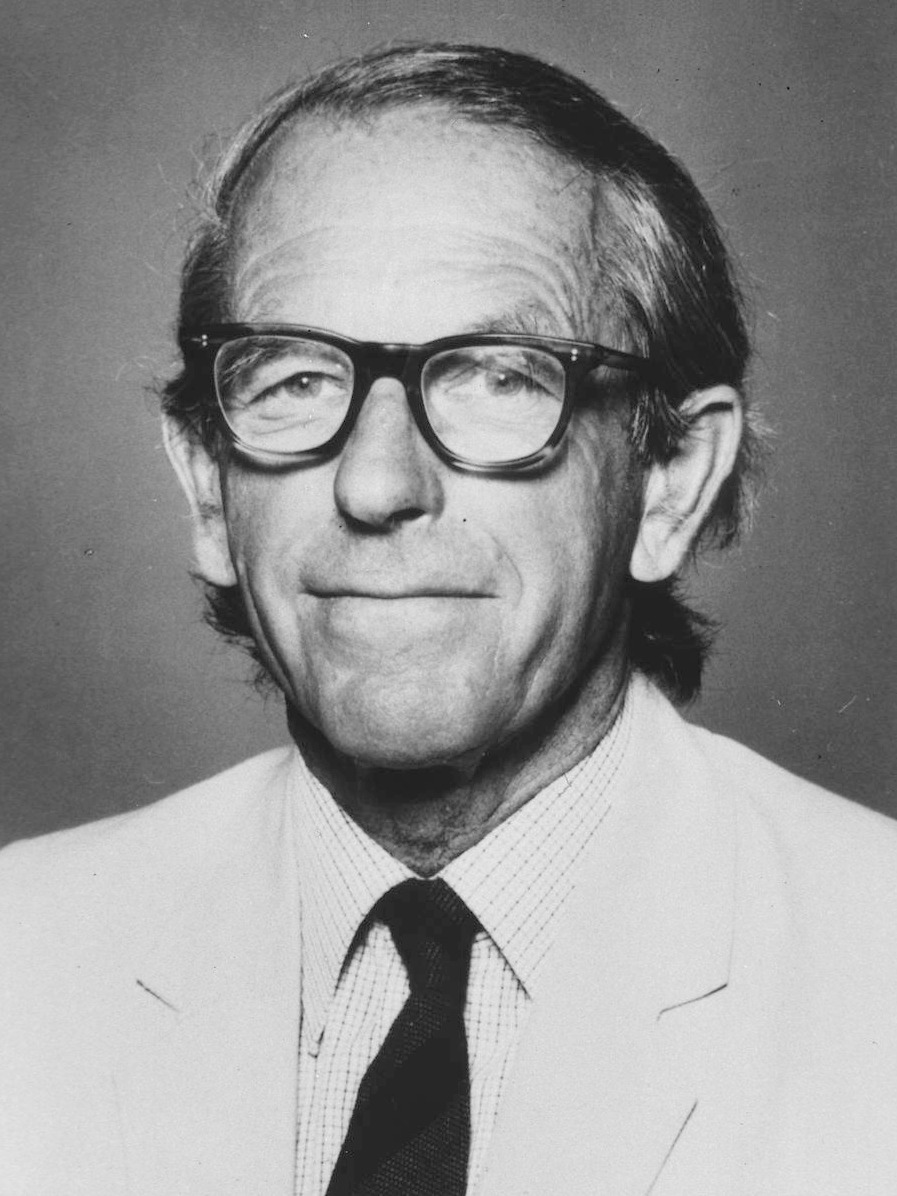
\includegraphics[width=0.30\linewidth]{images/book5/sanger.jpg}\hspace{0.04\linewidth}
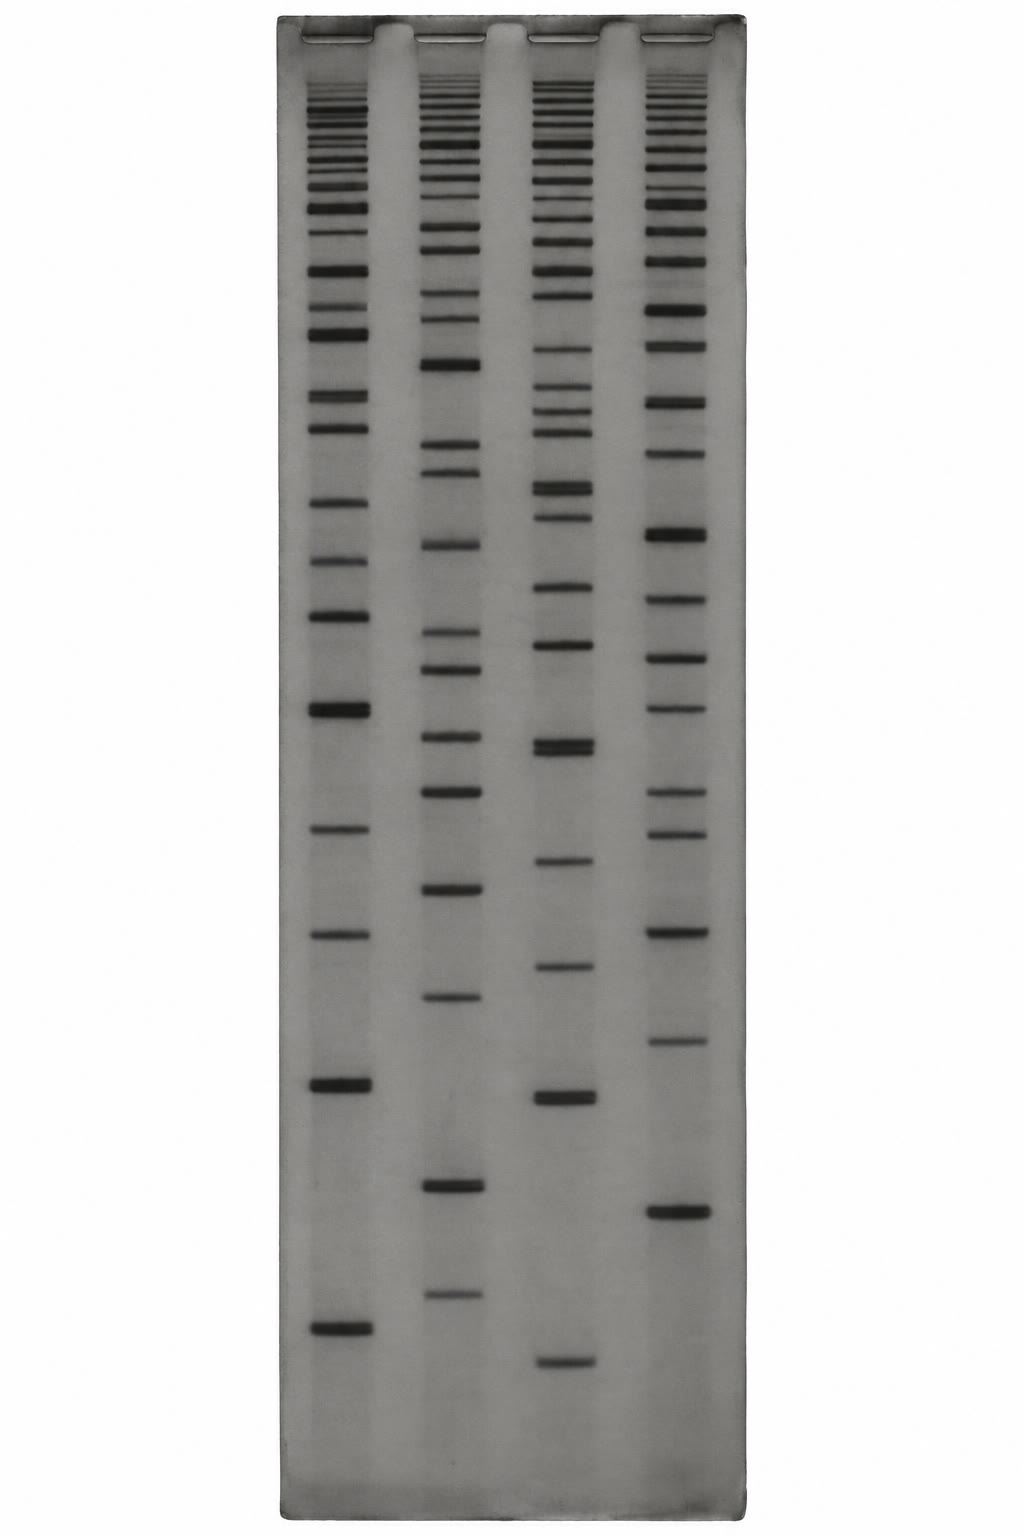
\includegraphics[width=0.30\linewidth]{images/book5/ai/b5-04-sanger-gel.jpg}

{\small يسارًا: فريدريك سانغر، الذي وضع أول طريقتين عمليتين \omterm{def:b3:genomics:ngs}{لقراءة}
البروتينات وDNA ونال جائزة نوبل عن كل منهما. يمينًا: صورة إشعاعية
ذاتية لهلام تسلسل من عهد ما قبل الشعيرات، مسرب لكل قاعدة، ويُقرأ
التسلسل صعودًا من سلّم الحزم.}
\end{omfigure}

\begin{omfigure}
\begin{tikzpicture}[every node/.style={font=\scriptsize}, >=stealth]
  % template and primer
  \draw[very thick, omDef] (0,3.0) -- (6,3.0); \node[left] at (-0.1,3.0) {القالب 3$'$};
  \node[right] at (6.05,3.0) {5$'$};
  \foreach \x/\b in {0.6/T,1.2/G,1.8/A,2.4/C,3.0/T,3.6/T,4.2/G,4.8/C} \node[above, omDef] at (\x,3.05) {\b};
  \draw[very thick, omProp] (0,2.6) -- (0.3,2.6); \node[left] at (-0.1,2.6) {البادئة};
  % terminated products
  \foreach \i/\len/\col/\b in {1/0.6/omDef/A, 2/1.2/omMeth/C, 3/1.8/omThm/T, 4/2.4/omExo/G, 5/3.0/omDef/A, 6/3.6/omDef/A, 7/4.2/omMeth/C, 8/4.8/omExo/G} {
    \draw[very thick, omProp] (0,2.6-0.32*\i) -- (\len-0.15,2.6-0.32*\i);
    \fill[\col] (\len-0.05,2.6-0.32*\i) circle (0.1);
    \node[right, \col] at (\len+0.05,2.6-0.32*\i) {dd\b};
  }
  \node[below, align=center] at (2.4,-0.25) {ناتج واحد لكل موضع، ينتهي كل منها\\بقاعدة ثنائية منزوعة الأكسجين متألقة};
  % capillary readout
  \draw[->, thick] (6.5,1.3) -- (7.4,1.3) node[midway, above] {الحجم};
  \draw[thick] (7.6,0.0) rectangle (11.6,2.6);
  \foreach \i/\col in {1/omDef, 2/omMeth, 3/omThm, 4/omExo, 5/omDef, 6/omDef, 7/omMeth, 8/omExo} {
    \draw[very thick, \col] (7.6+0.45*\i,0.1) .. controls (7.6+0.45*\i-0.15,0.1) and (7.6+0.45*\i-0.1,1.6) .. (7.6+0.45*\i,1.6) .. controls (7.6+0.45*\i+0.1,1.6) and (7.6+0.45*\i+0.15,0.1) .. (7.6+0.45*\i+0.3,0.1);
  }
  \foreach \i/\b in {1/A, 2/C, 3/T, 4/G, 5/A, 6/A, 7/C, 8/G} \node[above] at (7.6+0.45*\i,1.7) {\b};
  \node[below] at (9.6,-0.05) {الأقصر $\to$ الأطول: التسلسل، مقروءًا بالألوان};
\end{tikzpicture}

{\small التسلسل \omterm{def:b3:genomics:sanger}{بإنهاء السلسلة}. تنهي القاعدة ثنائية منزوعة الأكسجين
النسخةَ عند كل موضع تُدخل فيه؛ وتُفصل القطع، واحدة لكل طول،
بالحجم، ويُقرأ لون كل قاعدة طرفية بالترتيب.}
\end{omfigure}

\begin{definition}[التسلسل المتوازي الواسع]\label{def:b3:genomics:ngs}
\index{تسلسل بالتركيب}\index{قراءة}\index{تسلسل القراءات الطويلة}\index{مسام نانوي}
تقرأ أجهزة الجيل الثاني ملايين إلى مليارات القطع دفعةً واحدة. ففي
\emph{التسلسل بالتركيب} تُربط القطع، وقد وُصلت بها مهايئات عند
نهاياتها، بخلية تدفق زجاجية وتُضخَّم في موضعها عناقيدَ من جزيئات
متطابقة؛ ثم تُستطال العناقيد قاعدةً واحدة في كل دورة بنوكليوتيدات
متألقة محجوبة حجبًا عكوسًا، وتُصوَّر، ويُرفع الحجب، وتُستطال مجددًا،
فتضيف كل دورة قاعدةً إلى \emph{قراءة} كل عنقود. وطول القراءات
\qtyrange{100}{300}{bp}، وتؤخذ عادةً من طرفي القطعة
(\emph{نهايتان مزدوجتان})، بمعدل خطأ نحو $10^{-3}$ لكل قاعدة،
ويعطي الشوط الواحد ما يصل إلى $10^{12}$ قاعدة. أما أجهزة الجيل
الثالث \emph{ذات القراءات الطويلة} فتقرأ جزيئات مفردة بلا
تضخيم: إما بمراقبة بوليميراز واحد وهو يدخل نوكليوتيدات
متألقة في الزمن الحقيقي، وإما بتمرير DNA عبر \emph{مسام نانوي}
بروتيني وتسجيل التيار الأيوني الذي يعدّله كل تسلسل من
القواعد على نحوه الخاص. والقراءات بطول \qtyrange{10}{100}{kb} وأكثر
تعبر التكرارات التي تعجز عنها القراءات القصيرة، بمعدل خطأ خام أعلى
يخفضه التوافق.
\end{definition}

\begin{omfigure}
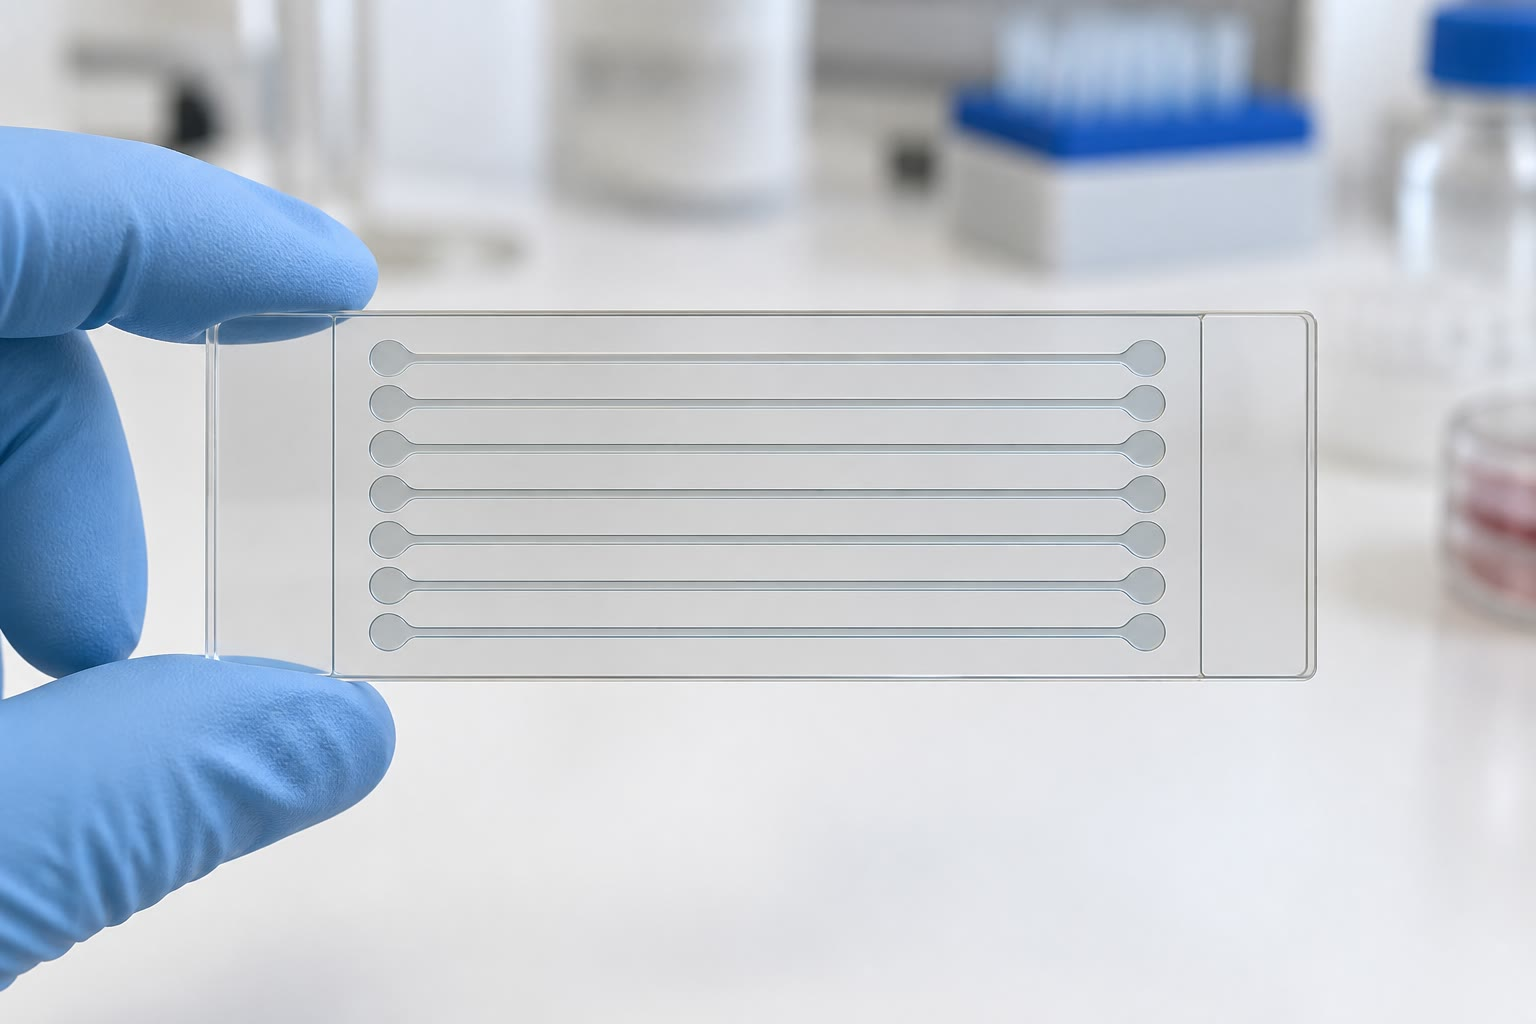
\includegraphics[width=0.46\linewidth]{images/book5/ai/b5-04-flowcell.jpg}\hspace{0.04\linewidth}
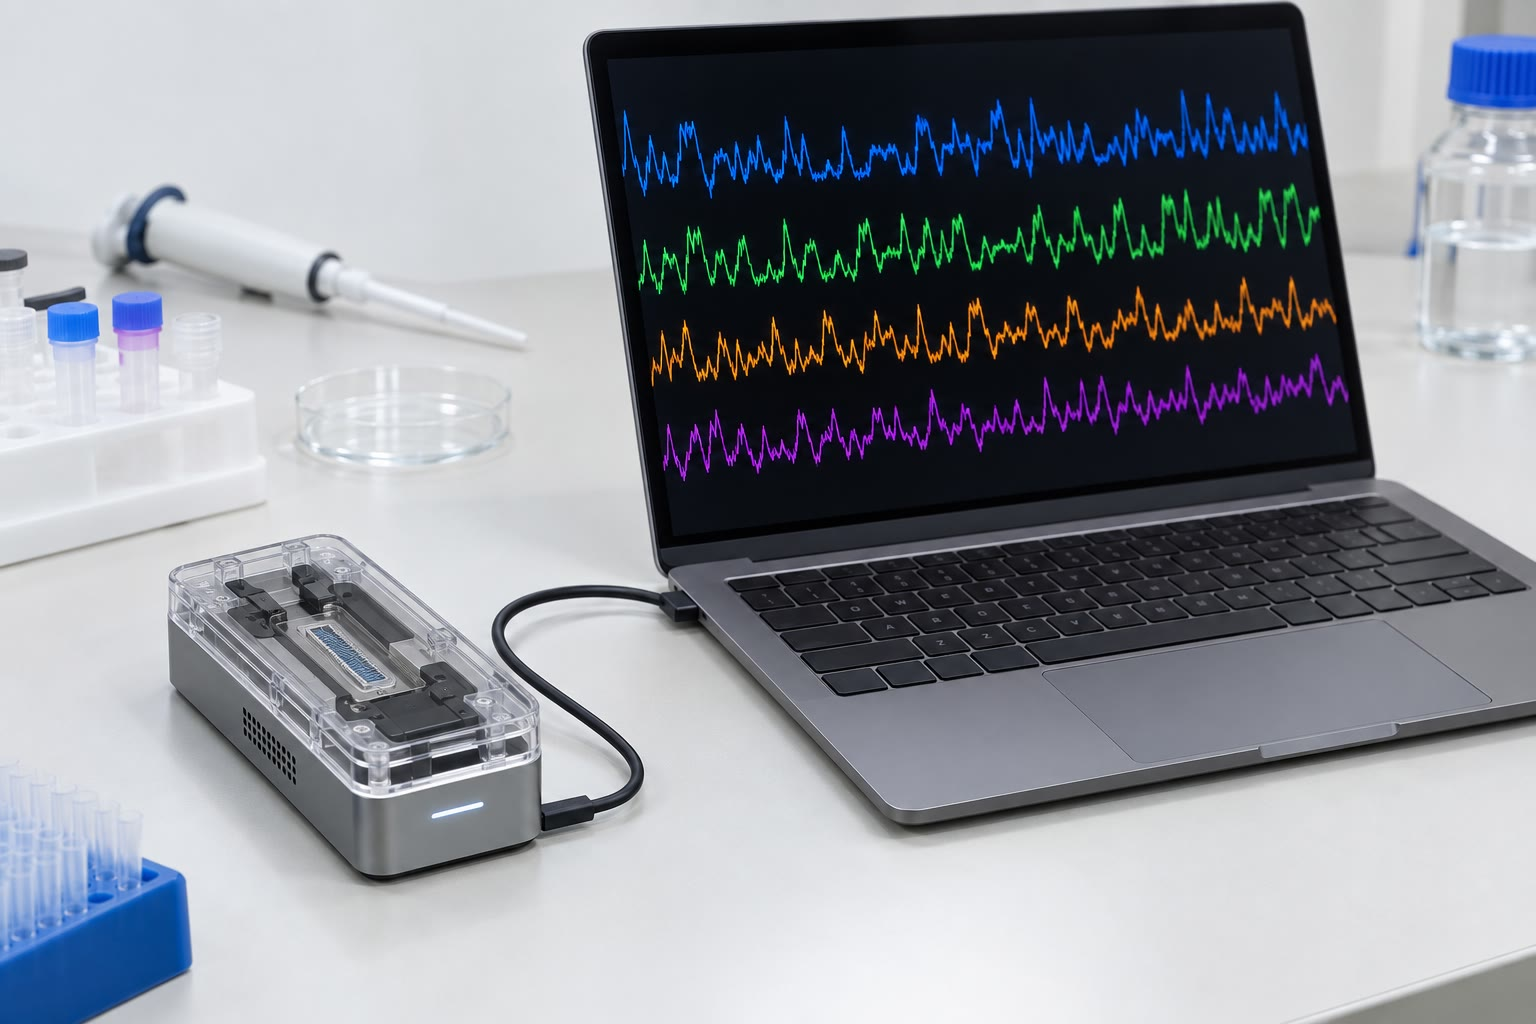
\includegraphics[width=0.46\linewidth]{images/book5/ai/b5-04-nanopore.jpg}

{\small يسارًا: خلية تدفق، وهي الشريحة الزجاجية التي تُنمّى عليها
مليارات عناقيد DNA وتُقرأ قاعدةً في كل دورة. يمينًا: مسلسل \omterm{def:b3:genomics:ngs}{بمسام
نانوي} بحجم الجيب يقرأ جزيئات مفردة بوصفها تغيرات في تيار
أيوني.}
\end{omfigure}

\begin{theorem}[التغطية والفجوات في مشروع خردقة]\label{thm:b3:genomics:lander-waterman}
\index{تغطية}\index{لاندر--ووترمان}\index{كونتيغ}
لتؤخذ $N$ \omterm{def:b3:genomics:ngs}{قراءة} طولها $L$ عند مواضع عشوائية على امتداد
جينوم طوله $G$، وليكن $c = NL/G$ هو \emph{التغطية}، أي
المتوسط العددي للقراءات التي تغطي قاعدةً واحدة. عندئذٍ تغطي قاعدةً
معينة قراءاتٌ عددها بواسوني بمتوسط $c$: فتكون نسبة
الجينوم التي لم تُسلسل
\[
P(\text{غير مغطى}) = e^{-c},
\]
وإذا لم يُعدّ تداخل قراءتين معترفًا به إلا إذا اشتركتا في
$T$ قاعدة على الأقل، بحيث $\theta = T/L$، كان العدد المتوقع من
\emph{الكونتيغات} (جزر القراءات المتداخلة)
\[
\text{الكونتيغات} = N\,e^{-c(1-\theta)},
\]
ويكون متوسط طولها $L\,\bigl(e^{c(1-\theta)} - 1\bigr)/c + L\theta$،
بالتقريب.
\end{theorem}
\begin{proof}
تقع نقاط بدء القراءات عشوائيًا بكثافة $N/G$ لكل قاعدة. وتغطي القاعدةَ
القراءاتُ التي تبدأ في $L$ قاعدة قبلها؛ وعدد
البدايات في نافذة طولها $L$ بواسوني بمتوسط $LN/G
= c$، واحتمال ألا توجد أي بداية هو $e^{-c}$. وتكون \omterm{def:b3:genomics:ngs}{القراءة} أقصى
كونتيغها يمينًا إذا لم تبدأ \omterm{def:b3:genomics:ngs}{قراءة} أخرى ضمن $L - T = L(1-\theta)$
قاعدة بعد بدايتها هي (\omterm{def:b3:genomics:ngs}{فالقراءة} التي تبدأ بعد ذلك تتداخل معها
بأقل من $T$ فلا تُوصل بها)؛ وذلك الاحتمال هو $e^{-c(1-\theta)}$،
ولأن لكل كونتيغ قراءةً واحدة بالضبط هي أقصاه يمينًا، يكون العدد
المتوقع من الكونتيغات $N e^{-c(1-\theta)}$. أما متوسط طول الكونتيغ
فينتج من قسمة $G$ على عدد الكونتيغات، مصحّحًا بنسبة
ما لم يُغطَّ.
\end{proof}

\begin{example}[كم يكفي]\label{ex:b3:genomics:coverage}
عند $c = 5$ تكون النسبة غير المسلسلة $e^{-5} = 0.7\,\%$ --- أي في
جينوم قدره \qty{3.2}{Gb}، عشرون مليون قاعدة في عشرات الآلاف من
الفجوات. وعند $c = 10$ تصير $4.5\times 10^{-5}$، أي \qty{150}{kb} جملةً.
وتُسلسل الجينومات البشرية عادةً عند $c = 30$ لا بسبب فجوات
التغطية ($e^{-30} \approx 10^{-13}$) بل لأن كل قاعدة يجب أن
تُقرأ مرات عدة على كل من الصبغيين لتُستدعى بثقة
متغايرة اللواقح في مواجهة معدل خطأ قدره $10^{-3}$
لكل \omterm{def:b3:genomics:ngs}{قراءة}. وتُسلسل الجينومات البكتيرية عند $c = 50$--$100$
للسبب نفسه ولأن ذلك رخيص. وتبيّن الصيغة أيضًا ما لا تصلحه
التغطية: فالتكرار الأطول من \omterm{def:b3:genomics:ngs}{القراءة} موضعٌ يتفرع عنده بيان
التداخل، ولا يحله أي قدر من القراءات القصيرة. ولهذا وُجدت
القراءات الطويلة.
\end{example}

\begin{omfigure}
\begin{tikzpicture}
\begin{axis}[
  width=0.7\linewidth, height=5.6cm,
  axis x line=bottom, axis y line=left,
  xmin=0, xmax=12, ymin=0.000001, ymax=1, ymode=log,
  xlabel={التغطية $c$}, ylabel={النسبة},
  xlabel style={font=\small, at={(axis description cs:0.5,-0.12)}, anchor=north},
  ylabel style={font=\small},
  tick label style={font=\small}, xtick={0,2,4,6,8,10,12},
  clip=false,
]
\addplot[very thick, omDef, domain=0:12, samples=40] {exp(-x)};
\addplot[very thick, omThm, domain=0.3:12, samples=40] {exp(-x*0.8)*x/12};
\node[font=\scriptsize, omDef, anchor=north west] at (axis cs:0.3,0.002) {النسبة غير المغطاة $e^{-c}$};
\node[font=\scriptsize, omThm, anchor=south west] at (axis cs:5.5,0.03) {كونتيغات لكل قراءة $\times\, c/12$، $\theta = 0.2$};
\end{axis}
\end{tikzpicture}

{\small مقدارا لاندر--ووترمان في مقابل التغطية: نسبة الجينوم التي لا
تُقرأ قط تهبط مثل $e^{-c}$، وعدد الكونتيغات (مقيسًا هنا لكل \omterm{def:b3:genomics:ngs}{قراءة})
يبلغ ذروته عند تغطية منخفضة ثم يهبط مع اندماج
الجزر.}
\end{omfigure}

\section{من القراءات إلى جينوم}

\begin{definition}[التجميع والتوصيف]\label{def:b3:genomics:assembly}
\index{تجميع}\index{سقالة}\index{N50}\index{توصيف}\index{جينوم مرجعي}
\emph{التجميع} يعيد بناء الجينوم من قراءاته بالتداخل: ففي
\emph{بيان التداخل} تكون كل \omterm{def:b3:genomics:ngs}{قراءة} عقدةً موصولةً بالقراءات التي
تتداخل معها؛ وفي \emph{بيان دي بروين}، المستعمل لمليارات القراءات
القصيرة، تكون كل قطعة بطول $k$ (متتالية جزئية طولها $k$) عقدةً ويكون
الجينوم مسلكًا خلالها. ويكسر البيانين كليهما تكرارٌ أطول من
\omterm{def:b3:genomics:ngs}{القراءة}، فيعطي مسالك متفرعة. ثم تُرتَّب الكونتيغات وتُوجَّه
في \emph{سقالات} بالقراءات مزدوجة النهايات وبمعلومات بعيدة المدى
(قراءات طويلة، وخرائط بصرية، وخرائط تماس صبغي)، وتوضع
السقالات على الصبغيات. وتُلخَّص جودة التجميع بمقياس
\emph{N50}: وهو طول الكونتيغ الذي يقع عنده نصف القواعد المجمّعة
في كونتيغات لا تقل عنه. ثم يجد \emph{التوصيف}
المورّثات: في البكتيريا بأطر \omterm{def:b3:genomics:ngs}{القراءة} المفتوحة الأطول من المصادفة؛ وفي
حقيقيات النوى بجمع إشارات التسلسل (مواقع التشذيب، والمروّجات،
وانحياز الرامزات)، والتماثل مع بروتينات معروفة، والنسخ المسلسلة
من RNA. والحصيلة، لنوع ما، \emph{جينوم مرجعي} تُحاذى
إليه كل \omterm{def:b3:genomics:ngs}{قراءة} لاحقة من ذلك النوع بدل أن تُجمَّع من
جديد.
\end{definition}

\begin{method}[من عينة إلى متغايرات]\label{met:b3:genomics:pipeline}
\index{استدعاء المتغايرات}
لدراسة إعادة تسلسل فرد في مواجهة مرجع: (1)
استخلص DNA، وجزّئه إلى \qtyrange{300}{500}{bp}، وصِل به مهايئات
(وهي \emph{المكتبة})؛ (2) سلسِل إلى التغطية المطلوبة (30$\times$
لجينوم بشري، و100$\times$ لإكسوم يلتقط
\qty{1.5}{\%} من الجينوم المشفِّرة للبروتين)؛ (3) حاذِ كل
\omterm{def:b3:genomics:ngs}{قراءة} إلى المرجع متسامحًا مع عدم التوافق؛ (4) عند كل موضع
عُدّ القواعد في القراءات: فالموضع الذي يخالف فيه نحو نصف القراءات
المرجعَ \emph{متغاير} متغاير اللواقح، والذي يخالفه فيه
جميعها تقريبًا متغاير متماثل اللواقح، والذي يخالفه فيه القليل خطأ؛
(5) رشّح بالعمق وجودة القاعدة وتوازن الطاقين؛ (6) وصّف كل
متغاير بأثره في أي مورّثة (مرادف، أو مغيّر للمعنى، أو معدِم، أو
تشذيبي، أو مزيح للإطار) وبتواتره في قواعد بيانات الجمهرات؛ (7)
وللتشخيص، أبقِ المتغايرات النادرة المتوقَّع ضررها في مورّثات
تتسق مع النمط الظاهري، وأكّدها \omterm{def:b3:genomics:sanger}{بتسلسل سانغر}.
\end{method}

\section{كيف تبدو الجينومات}

\begin{proposition}[حجم الجينوم وعدد المورّثات]\label{prop:b3:genomics:sizes}
\index{مفارقة القيمة C}\index{حجم الجينوم}
تمتد أحجام الجينومات على عامل قدره $10^{5}$ بين حقيقيات النوى ---
\qty{12}{Mb} للخميرة، و\qty{100}{Mb} للدودة، و\qty{140}{Mb}
للذبابة، و\qty{3.2}{Gb} للإنسان، و\qty{16}{Gb} للبصل،
و\qty{130}{Gb} لسمكة الرئة، و\qty{150}{Gb} لزنبقة \emph{Paris
japonica} --- بينما لا تمتد أعداد المورّثات إلا على عامل قدره $10$:
\num{6000} في الخميرة، و\num{20000} في الدودة، و\num{14000} في الذبابة،
ونحو \num{20000} مورّثة مشفِّرة للبروتين في الإنسان، و\num{40000} في الأرز.
وهذه هي \emph{\omterm{prop:b3:genomics:sizes}{مفارقة القيمة C}}: \omterm{prop:b3:genomics:sizes}{فحجم الجينوم} لا يقيس
التعقيد، ولا يقيسه عدد المورّثات. وإنما يتغير المحتوى غير المشفِّر
--- الإنترونات والعناصر القافزة والتكرارات الساتلة --- ويتضاعف
عدد البروتينات التي يستطيع جينوم إنتاجها أضعافًا فوق عدد مورّثاته
بالتشذيب البديل (\cref{ch:b3:rna-regulation})
وبالتنظيم، وهناك يُكتب تعقيد الكائن في معظمه. أما الجينومات
البكتيرية فمرصوصة، وحجمها يتبع عدد المورّثات فعلًا: نحو مورّثة
لكل كيلوقاعدة، و\qty{88}{\%} منها مشفِّرة في \emph{E.~coli}.
\end{proposition}

\begin{example}[الجينوم البشري بحسب محتواه]\label{ex:b3:genomics:content}
من \qty{3.2}{Gb}: الإكسونات المشفِّرة للبروتين \qty{1.5}{\%}؛
والإنترونات والمناطق غير المترجمة من المورّثات نحو \qty{35}{\%}؛
والعناصر القافزة وحفرياتها نحو \qty{45}{\%} --- فالنواقل الرجعية
LINE-1 \qty{17}{\%}، وعناصر Alu \qty{10}{\%} (أكثر من مليون نسخة من
تسلسل بطول \qty{300}{bp})، والفيروسات الرجعية الداخلية \qty{8}{\%}؛
والمضاعفات القطعية \qty{5}{\%}؛ والتكرارات البسيطة والسواتل، ومنها
القسيمات المركزية، نحو \qty{5}{\%}؛ والباقي تسلسل فريد غير مشفِّر،
حيث تسكن العناصر المنظِّمة. وما تزال \numrange{100}{200} مورّثة
تشفّر آلة LINE-1 فاعلة، وتقع إدخالات جديدة نحو
مرة في كل عشرين ولادة. ونحو \qty{8}{\%} من الجينوم تحت انتقاء
تنقية قابل للكشف --- وهو أكثر بكثير من الإكسونات --- ومعظم
ذلك تنظيمي.
\end{example}

\begin{omfigure}
\begin{tikzpicture}[every node/.style={font=\scriptsize}]
  \def\w{12}
  % stacked bar: fractions
  \fill[omThm] (0,0) rectangle (0.18,0.7);
  \fill[omDef!60] (0.18,0) rectangle (4.38,0.7);
  \fill[omProp!70] (4.38,0) rectangle (6.42,0.7);
  \fill[omProp!45] (6.42,0) rectangle (7.62,0.7);
  \fill[omProp!25] (7.62,0) rectangle (9.78,0.7);
  \fill[omMeth!50] (9.78,0) rectangle (10.38,0.7);
  \fill[gray!45] (10.38,0) rectangle (10.98,0.7);
  \fill[gray!15] (10.98,0) rectangle (12,0.7);
  \draw[thick] (0,0) rectangle (12,0.7);
  % labels above/below with leaders
  \draw (0.09,0.7) -- (0.09,1.1); \node[above, align=center] at (0.5,1.1) {إكسونات\\\qty{1.5}{\%}};
  \node[above] at (2.3,0.75) {إنترونات ومناطق غير مترجمة: \qty{35}{\%}};
  \node[below, align=center] at (5.4,-0.05) {LINE-1\\\qty{17}{\%}};
  \node[below, align=center] at (7.0,-0.05) {Alu\\\qty{10}{\%}};
  \node[below, align=center] at (8.7,-0.05) {عناصر قافزة أخرى،\\فيروسات رجعية \qty{18}{\%}};
  \node[above, align=center] at (10.1,0.75) {مضاعفات\\قطعية \qty{5}{\%}};
  \node[below, align=center] at (10.7,-0.05) {سواتل\\\qty{5}{\%}};
  \draw[gray] (11.5,0.72) -- (12.0,1.05); \node[above, align=center] at (12.3,1.05) {تسلسل فريد آخر\\غير مشفِّر};
  \draw[decorate, decoration={brace, amplitude=4pt, mirror}] (4.38,-1.0) -- (9.78,-1.0) node[midway, below=4pt] {مشتق من عناصر قافزة: \qty{45}{\%}};
\end{tikzpicture}

{\small الجينوم البشري بحسب محتواه، بالمقياس. فالإكسونات المشفِّرة
للبروتين (بالأحمر) شظية؛ ونحو نصف الجينوم منحدر من
عناصر قافزة.}
\end{omfigure}

\begin{definition}[الجينوميات المقارنة]\label{def:b3:genomics:comparative}
\index{متماثل متعامد}\index{متماثل متوازٍ}\index{تصاحب المواضع}\index{عنصر غير مشفِّر محفوظ}\index{مضاعفة الجينوم الكاملة}
المورّثتان في نوعين المنحدرتان من مورّثة واحدة في سلفهما المشترك
\emph{متماثلتان متعامدتان}؛ والمورّثتان داخل نوع واحد المنحدرتان من
مضاعفة \emph{متماثلتان متوازيتان}. وكتل الصبغيات التي يُحفظ فيها
ترتيب المورّثات بين نوعين \emph{متصاحبة}؛ ويتيح التصاحب أن
تُحدَّد مورّثة في جينوم من موضعها في آخر، ويكشف
إعادات الترتيب التي تفصل نمطين صبغيين (نحو \num{1000}
بين الإنسان والفأر). والمتتاليات المحفوظة عبر أنواع متباعدة
التي لا تشفّر بروتينًا --- وهي \emph{العناصر غير المشفِّرة المحفوظة}،
وبعضها محفوظ حفظًا فائقًا حتى القاعدة على امتداد \qty{200}{bp} بين الإنسان
والسمكة --- معزِّزات لمورّثات تطورية في معظمها. و\emph{مضاعفات
الجينوم الكاملة} وسمت تاريخ سلالات بعينها: جولتان عند
أصل الفقاريات (فعناقيد Hox الأربعة في الثدييات مقابل عنقود واحد
في اللافقاريات)، وواحدة في سلف السلمونيات، وواحدة في سلالة
الخميرة، وعدة في النباتات الزهرية؛ وتُفقد المورّثات المضاعفة في
معظمها على مدى عشرات ملايين السنين، وتتباعد الناجيات في
الوظيفة.
\end{definition}

\begin{example}[الإنسان والشمبانزي]\label{ex:b3:genomics:chimp}
يختلف التسلسل المحاذى وحيد النسخة بين الإنسان والشمبانزي في
\qty{1.2}{\%} من القواعد --- أي نحو \num{35} مليون تبدّل --- وفي
إقحامات وحذوف تبلغ معًا \qty{3}{\%} أخرى من كل
جينوم. ويختلف إنسانان عند نحو قاعدة واحدة من كل
ألف، أي نحو \numrange{4}{5} ملايين موضع، مع بضعة آلاف من
المتغايرات البنيوية؛ ويختلف شمبانزيان، وجمهرتهما أكبر منذ
زمن أطول، أكثر من ذلك. ويحمل الطفل نحو \num{70} طفرة
جديدة غائبة عن والديه معًا، أربعة أخماسها من
الأب، ويرتفع العدد نحو اثنتين لكل سنة من عمر الأب ---
وهو حساب \cref{ch:b3:dna-repair} مطبقًا على انقسامات
تكوين النطاف الكثيرة.
\end{example}

\section{الجينومات والصفات}

\begin{definition}[الارتباط على مستوى الجينوم]\label{def:b3:genomics:gwas}
\index{دراسة الارتباط على مستوى الجينوم}\index{تعدد الأشكال أحادي النوكليوتيد}\index{درجة متعددة المورّثات}
\emph{تعدد الأشكال أحادي النوكليوتيد} (SNP) موضع تَرِد فيه
قاعدتان كل منهما في \qty{1}{\%} من الجمهرة على الأقل؛ ونحو
عشرة ملايين منها شائعة في البشر. و\emph{دراسة الارتباط على مستوى
الجينوم} (GWAS) تحدد أنماط مئات الآلاف من مواضع SNP في آلاف
من المصابين بمرض وآلاف من غير المصابين، وتسأل عند كل موضع
هل يكون أحد الأليلين أكثر تواترًا في الحالات. ولأن مليون
اختبار يُجرى، لا تُعتدّ النتيجة إلا دون عتبة دلالة
قدرها نحو $5\times 10^{-8}$ ($0.05$ مقسومًا على المليون اختبار
المستقل فعليًا). والمواضع المرتبطة تعلّم منطقة لا متغايرًا
سببيًا، لأن الأليلات المتجاورة تنتقل معًا (عدم الاتزان
الارتباطي) على مدى عشرات الكيلوقواعد. وفي معظم الأمراض الشائعة
تزيح الأليلات المرتبطة الخطرَ بضعة في المئة وتقع في
التسلسل المنظِّم غالبًا؛ وأثرها المجموع، مضافًا على آلاف
المواضع بوصفه \emph{درجة متعددة المورّثات}، يفسر جزءًا من
التوريث ويتنبأ بالخطر تنبؤًا يقارب تنبؤ التاريخ العائلي.
\end{definition}

\begin{remark}[ما أنجزته الجينوميات وما لم تنجزه]\label{rem:b3:genomics:delivered}
كان التسلسل حاسمًا حيث تكون لمورّثة واحدة أثر كبير:
فآلاف الأمراض المندلية عُرفت مورّثاتها، ويعطي تسلسل
إكسوم طفل باضطراب غير مشخَّص تشخيصًا في
نحو ثلث الحالات. وتكشف جينومات السرطان أي المورّثات القائدة يحمل
ورمٌ وأي الأدوية قد تنجع (\cref{ch:b3:cancer-biology})؛
وتتتبع جينومات الممرضات الفاشيات سلالةً سلالة
(\cref{ch:b3:bacteriology})؛ وأعادت الجينومات القديمة كتابة ما قبل
التاريخ البشري، إذ بيّنت أن من هم خارج إفريقيا يحملون نحو \qty{2}{\%}
من DNA النياندرتال. أما الأمراض الشائعة --- السكري وداء القلب
والفصام --- فقد أعطت الجينوميات فيها آلاف الآثار الصغيرة و
آليات قليلة، وما يزال وعد التنبؤ من جينوم شخص
سليم متواضعًا. فالجينوم قائمة أجزاء؛ أما
بيولوجيا تفاعل الأجزاء فلا تُقرأ منه.
\end{remark}

\section{تمارين}

\begin{exercise}[$\star$]\label{exo:b3:genomics:1}
فسّر لماذا ينهي النوكليوتيد \omterm{def:b3:genomics:sanger}{ثنائي منزوع الأكسجين} سلسلة DNA النامية،
ولماذا يجب أن يحوي تفاعل سانغر الصورتين السوية وثنائية منزوعة
الأكسجين من كل نوكليوتيد.
\end{exercise}

\begin{exercise}[$\star$]\label{exo:b3:genomics:2}
يعطي شوط $4\times 10^{8}$ \omterm{def:b3:genomics:ngs}{قراءة} مزدوجة بطول $2\times \qty{150}{bp}$.
فما التغطية التي يعطيها لجينوم بشري قدره \qty{3.2}{Gb}؟ ولجينوم
بكتيري قدره \qty{5}{Mb}؟
\end{exercise}

\begin{exercise}[$\star$]\label{exo:b3:genomics:3}
عرّف الكونتيغ \omterm{def:b3:genomics:assembly}{والسقالة} ومقياس \omterm{def:b3:genomics:assembly}{N50}. \omterm{def:b3:genomics:assembly}{تجميع} قدره \qty{100}{Mb} فيه عشرة
كونتيغات بطول \qty{8}{Mb} و\num{2000} بطول \qty{10}{kb}. فما مقياس \omterm{def:b3:genomics:assembly}{N50} فيه؟
\end{exercise}

\begin{exercise}[$\star$]\label{exo:b3:genomics:4}
اذكر \omterm{prop:b3:genomics:sizes}{مفارقة القيمة C} بمثالين، وقل ما الذي يفسّر في معظمه فائض DNA في
الجينومات الكبيرة.
\end{exercise}

\begin{exercise}[$\star\star$]\label{exo:b3:genomics:5}
باستعمال \cref{thm:b3:genomics:lander-waterman}، أوجد التغطية اللازمة
لألا تبقى أكثر من قاعدة واحدة من كل مليون بلا تسلسل، والعدد المتوقع
من الكونتيغات لجينوم قدره \qty{5}{Mb} يُقرأ عند $c = 8$ بقراءات
بطول \qty{150}{bp} وأقل تداخل \qty{30}{bp}.
\end{exercise}

\begin{exercise}[$\star\star$]\label{exo:b3:genomics:6}
متغاير متغاير اللواقح تغطيه $30$ \omterm{def:b3:genomics:ngs}{قراءة}. بفرض أن كل \omterm{def:b3:genomics:ngs}{قراءة}
تُظهر أحد الأليلين باحتمال $1/2$، فما احتمال
أن تُظهر أقل من $8$ قراءات الأليلَ المتغاير (فيُظنّ خطأً أنه
أخطاء)؟ استعمل تقريبًا سويًا بمتوسط $15$ وانحراف
معياري $\sqrt{7.5}$. ولماذا تكون $30\times$ هي المعيار؟
\end{exercise}

\begin{exercise}[$\star\star$]\label{exo:b3:genomics:7}
جينوم فيه تكرار بطول \qty{6}{kb} حاضر في \num{500} نسخة.
فسّر لماذا ينهار في \omterm{def:b3:genomics:assembly}{تجميع} من قراءات بطول \qty{150}{bp}، وكيف يبدو
البيان الناتج، وأي طول \omterm{def:b3:genomics:ngs}{قراءة} يحلّه.
\end{exercise}

\begin{exercise}[$\star\star$]\label{exo:b3:genomics:8}
يختلف إنسانان عند قاعدة واحدة من كل ألف. فكم اختلافًا في
إكسوميهما (\qty{48}{Mb} من التسلسل المشفِّر)؟ وإذا كان ثلثا الاختلافات
المشفِّرة مرادفًا أو سليمًا والباقي يغيّر بروتينًا، فكم
متغايرًا مغيّرًا للبروتين يحمل شخص قياسًا إلى
آخر؟
\end{exercise}

\begin{exercise}[$\star\star$]\label{exo:b3:genomics:9}
تختبر دراسة ارتباط $10^{6}$ موضع SNP عند العتبة $p < 5\times 10^{-8}$.
فكم إيجابية كاذبة تُتوقع إذا لم يكن أي موضع مرتبطًا حقًا؟ وأليل
في موضع يرفع خطر مرض تواتره \qty{2}{\%} إلى
\qty{2.3}{\%}. فسّر لماذا يستحيل كشف أثر كهذا في دراسة على
ألف شخص ولماذا لا ينفع فردًا، ومع ذلك قد يدل
على آلية.
\end{exercise}

\begin{exercise}[$\star\star\star$]\label{exo:b3:genomics:10}
الجينومات البكتيرية نحو \qty{88}{\%} منها مشفِّرة؛ والجينوم البشري
\qty{1.5}{\%}. أعطِ ثلاث فرضيات --- جمهرية وراثية، وبنيوية،
وتنظيمية --- للفرق، ولكل منها مشاهدةً جينومية
تدعمها أو تضعفها.
\end{exercise}

\begin{exercise}[$\star\star\star$]\label{exo:b3:genomics:11}
اشتق عدد كونتيغات لاندر--ووترمان لقراءات مخلوطة بطولين مختلفين:
$N_{1}$ \omterm{def:b3:genomics:ngs}{قراءة} قصيرة بطول $L_{1}$ و$N_{2}$ \omterm{def:b3:genomics:ngs}{قراءة}
طويلة بطول $L_{2}$، مع عدّ التداخلات بالحد الأدنى $T$ نفسه.
(اعتبر كل \omterm{def:b3:genomics:ngs}{قراءة} أقصى كونتيغها يمينًا إذا لم تبدأ \omterm{def:b3:genomics:ngs}{قراءة} من أي
نوع ضمن طولها هي ناقص $T$.) وبيّن أن قراءات طويلة قليلة
تخفض عدد الكونتيغات أكثر مما يخفضه العدد نفسه من القواعد في
قراءات قصيرة.
\end{exercise}

\begin{exercise}[$\star\star\star$]\label{exo:b3:genomics:12}
يُحتجّ بأن عناقيد Hox الأربعة في الثدييات منحدرة من عنقود
واحد بجولتي مضاعفة للجينوم الكامل عند أصل
الفقاريات. اذكر أي نمط من المتماثلات المتوازية عبر الجينوم، وأي
نمط في جينومات اللمبريات وحبليات اللافقاريات، تتنبأ به
تلك الفرضية، وكيف يمكن تمييزها عن
مضاعفتين مستقلتين للعنقود وحده.
\end{exercise}

\section{مسألة: جينومان على جهاز واحد}

\begin{problem}[{مسألة نهاية الأسبوع --- بكتيريا وإنسان يُسلسلان في
الشوط نفسه: القراءات مقسومة، والتغطية والفجوات محسوبة،
والكونتيغات معدودة، والمتغايرات متغايرة اللواقح مستدعاة في مواجهة
معدل الخطأ، ومحتوى الجينوم البشري موزونًا، ودراسة ارتباط
مقدَّرة الحجم، وتنتهي إلى عدد الكونتيغات عند تغطية منخفضة، والتغطية
التي تجعل استدعاء المتغاير آمنًا، وعدد الطفرات الجديدة في
طفل}]
\label{pb:b3:genomics:1}
معطيات: يعطي شوط واحد $6\times 10^{8}$ \omterm{def:b3:genomics:ngs}{قراءة} بطول \qty{150}{bp}.
وجينوم بكتيري قدره \qty{4.6}{Mb}؛ والجينوم البشري \qty{3.2}{Gb}
(أحادي الصيغة). وأقل تداخل $T = \qty{30}{bp}$. ومعدل الخطأ $10^{-3}$
لكل قاعدة في \omterm{def:b3:genomics:ngs}{القراءة}. والتسلسل المشفِّر البشري \qty{48}{Mb}؛ والجينوم
\qty{45}{\%} منه مشتق من عناصر قافزة، مع $1.1$ مليون نسخة Alu بطول
\qty{300}{bp}. ويختلف إنسانان عند موضع واحد من \num{1000}. ومعدل
الطفرة $1.2\times 10^{-8}$ لكل قاعدة في الجيل.

\medskip
\noindent\textbf{الجزء الأول --- البكتيريا.}
\begin{enumerate}
  \item تُعطى البكتيريا \qty{0.2}{\%} من الشوط. فكم \omterm{def:b3:genomics:ngs}{قراءة}، وما
        التغطية؟
  \item ما نسبة جينومها التي لم تُسلسل؟ وكم قاعدة يبلغ
        ذلك؟
  \item احسب $\theta$ والعدد المتوقع من الكونتيغات.
  \item استعملت تجربة أولية سابقة \num{30000} \omterm{def:b3:genomics:ngs}{قراءة} فقط. فما التغطية،
        والنسبة غير المغطاة، وعدد الكونتيغات؟
  \item يحوي الجينوم \num{7} نسخ من أوبرون RNA ريبوزومي بطول
        \qty{5}{kb}. فسّر ما يحدث لها في \omterm{def:b3:genomics:assembly}{التجميع} وكم
        نهاية كونتيغ ينتج هذا وحده.
  \item للبكتيريا نحو مورّثة لكل كيلوقاعدة. فكم مورّثة،
        وإذا كان \qty{88}{\%} من الجينوم مشفِّرًا، فما متوسط طول
        المورّثة؟
\end{enumerate}

\medskip
\noindent\textbf{الجزء الثاني --- الإنسان.}
\begin{enumerate}[resume]
  \item يذهب باقي الشوط إلى جينوم بشري واحد. فما تغطية
        الجينوم ثنائي الصيغة لكل نسخة أحادية (أي مجموع القواعد
        مقسومًا على \qty{3.2}{Gb})؟
  \item عند موضع متغاير اللواقح يغطي كلًا من الأليلين
        نحو نصف القراءات. فبتغطية السؤال 7، ما العدد
        المتوقع من القراءات التي تُظهر كل أليل؟
  \item يُظهر الخطأ قاعدة خاطئة في \omterm{def:b3:genomics:ngs}{قراءة} باحتمال
        $10^{-3}$. فعند موضع متماثل اللواقح تغطيه $c$ \omterm{def:b3:genomics:ngs}{قراءة}، ما
        العدد المتوقع من القراءات التي تُظهر قاعدة خاطئة بعينها
        ($10^{-3}/3$ لكل منها)؟ ولماذا ترفض قاعدةُ ``استدعِ متغايرًا
        إذا أظهرته $3$ قراءات على الأقل و\qty{20}{\%} من القراءات على
        الأقل'' الأخطاءَ عند هذه التغطية؟
  \item كم موضعًا متغاير اللواقح يحمل الإنسان الواحد (فنصف
        الاختلافات بين جينومين عشوائيين يقع في كل منهما تقريبًا:
        خذ موضعًا واحدًا من \num{1500})؟ وكم في التسلسل المشفِّر؟
  \item تُحاذى القراءات إلى مرجع. فسّر لماذا تُحاذى القراءات الآتية
        من عناصر Alu إلى النسخة الخاطئة غالبًا وما
        نتيجة ذلك في \omterm{met:b3:genomics:pipeline}{استدعاء المتغايرات} داخلها.
  \item يُسلسل طفل مع والديه. فكم طفرة جديدة
        تتوقع؟ وكم \omterm{def:b3:genomics:ngs}{قراءة} في الطفل، عند هذه التغطية،
        يجب أن تُظهر متغايرًا غائبًا عن \emph{كلا} الوالدين حتى
        يُصدَّق، ولماذا تكون تغطية الوالدين بأهمية تغطية
        الطفل؟
  \item يلتقط مختبر سريري الإكسوم (\qty{48}{Mb})
        ويسلسله عند $100\times$. فكم \omterm{def:b3:genomics:ngs}{قراءة} يقتضي ذلك،
        ولماذا يكون أرخص لكل مريض من جينوم عند $28\times$
        مع أن تغطيته أعلى؟
\end{enumerate}

\medskip
\noindent\textbf{الجزء الثالث --- محتوى جينوم.}
\begin{enumerate}[resume]
  \item ما نسبة الجينوم البشري التي هي Alu، وما نسبة
        قراءات السؤال 7 الآتية من عناصر Alu؟
  \item المرجع \qty{3.2}{Gb} لكن الخلية ثنائية الصيغة تحمل
        \qty{6.4}{Gb}؛ وللبصل ذي \qty{16}{Gb} نحو \num{60000}
        مورّثة. فما النسبة المشفِّرة من جينوم البصل، إذا كان متوسط
        تسلسل مورّثاته المشفِّر \qty{1.5}{kb}؟
  \item يختلف الإنسان والشمبانزي في \qty{1.2}{\%} من القواعد المحاذاة.
        فكم تبدّلًا يبلغ ذلك في \qty{2.9}{Gb} من التسلسل القابل
        للمحاذاة؟ وإذا قُسم بالتساوي بين السلالتين على مدى $6.5$
        ملايين سنة، فأي معدل طفرة لكل قاعدة في السنة يقتضي ذلك،
        وكم لكل جيل من $25$ سنة؟ قارن بالقياس
        المباشر المعطى في المعطيات.
  \item مضاعفتان للجينوم في الفقاريات ينبغي أن تعطيا حتى أربع
        نسخ من كل مورّثة سلفية. وللإنسان نحو \num{20000}
        مورّثة، ولحبلي اللافقاريات \emph{Ciona} نحو
        \num{16000}. فما نسبة المضاعفات التي فُقدت، على
        فرض أن السلف كان له \num{16000}؟
  \item فسّر لماذا يكون عدد المورّثات مقياسًا رديئًا لتعقيد
        الكائن، مستعينًا بعدد أشكال التشذيب البديل في
        \cref{ch:b3:rna-regulation} حجةً.
  \item \qty{8}{\%} من الجينوم تحت انتقاء تنقية ولكن
        \qty{1.5}{\%} فقط تشفّر بروتينًا. فما الأرجح أن يكون
        الباقي، وكيف تختبر عنصرًا مرشحًا واحدًا؟
\end{enumerate}

\medskip
\noindent\textbf{الجزء الرابع --- دراسة ارتباط.}
\begin{enumerate}[resume]
  \item يُختبر $10^{6}$ موضع SNP. اذكر عتبة بونفيروني لخطأ
        عائلي قدره $0.05$، والعدد المتوقع من الإيجابيات
        الكاذبة عند $p < 10^{-5}$.
  \item مرض انتشاره \qty{1}{\%}. وأليل خطر تواتره
        $0.3$ يرفع الأرجحية \qty{5}{\%}. احسب خطر المرض
        عند حامل نسختين، وحامل نسخة واحدة، وغير الحامل، بأخذ
        خطر غير الحامل \qty{0.9}{\%}. (اضرب الأرجحيات.)
  \item وُجد مئتا أليل كهذا. فسّر ما \omterm{def:b3:genomics:gwas}{درجة تعدد المورّثات}،
        ولماذا قد توافق درجةُ شخص في أعلى \qty{1}{\%}
        خطرًا بعدة أضعاف مع أن كل أليل لا يكاد يفعل
        شيئًا.
  \item فسّر لماذا لا يكون الموضع الذي يبلغ الدلالة هو المتغاير
        السببي عادةً، وأي تجربة تحدد المتغاير السببي
        في المنطقة.
  \item جينوم قديم من عظم عمره \num{40000} سنة يُسلسل
        عند $c = 0.5$. فما نسبة ما يُقرأ منه؟ ولماذا يستطيع مع ذلك أن
        يجيب عن أسئلة في تاريخ الجمهرات لا يجيب عنها جينوم
        حديث وحده؟
  \item لخّص: عدد الكونتيغات في \omterm{def:b3:genomics:assembly}{التجميع} الأولي
        (السؤال~4)، والتغطية لكل جينوم أحادي الصيغة التي تعطي نحو
        $15$ \omterm{def:b3:genomics:ngs}{قراءة} لكل أليل (السؤالان~7--8)، وعدد الطفرات الجديدة
        في طفل (السؤال~12).
\end{enumerate}
\end{problem}
